% Fathom: Cognitive Geometry of Language Model Reasoning
% ICML 2026 Mechanistic Interpretability Workshop
% Neel Nanda, organizer. Papers due May 8, 2026.

\documentclass{article}
\usepackage{icml2026}
\usepackage[utf8]{inputenc}
\usepackage{amsmath,amssymb,amsfonts}
\usepackage{graphicx}
\usepackage{booktabs}
\usepackage{hyperref}
\usepackage{natbib}
\usepackage{xcolor}

% Look for figures both in paper-relative (./) and project-relative (../)
% directories so we can run pdflatex from the paper/ directory and still
% resolve images stored in the top-level figures/ folder. The
% \includegraphics calls already carry the figures/ prefix, so we only
% need to provide the directory that prefix is joined to.
\graphicspath{{./}{../}}

\title{Fathom: Cognitive Measurement Instruments for Transformer Internals \\
via SAE Feature Coherence Geometry}
\icmltitlerunning{Fathom: Cognitive Measurement Instruments}

\author{
  Alexander Rodabaugh \\
  Fathom Intelligence \\
  \texttt{flobi@darkflobi.com}
}

\begin{document}
\maketitle

% ══════════════════════════════════════════════════════════════
% ABSTRACT
% ══════════════════════════════════════════════════════════════
\begin{abstract}
We present Fathom, a suite of cognitive measurement instruments
for transformer internals built on sparse autoencoder (SAE) feature
coherence geometry. Our contributions span measurement, diagnosis,
and intervention:

\textit{Measurement.} We introduce commitment intensity ($S$), derived
as the inverse participation ratio (IPR) of per-token coherence events.
$S_\text{early}$ (first 7 tokens) discriminates hallucination from
correct generation with pooled $d = 0.494$ across three independent
designs (Fisher $p = 0.0008$), outperforms logit entropy head-to-head
(AUC $0.663$ vs.\ $0.607$), and replicates across two architecture
families (Fisher $p = 0.0006$). Three SAE-free probes across four
architectures all fail (Fisher $p > 0.6$).

\textit{Diagnosis.} We discover that the \textit{shape} of per-layer
coherence distributions carries discriminative information invisible
to scalar summaries. The Gini coefficient of coherence across layers
achieves AUC $= 0.685$ ($n = 200$, 13/16 metrics significant after
Holm--Bonferroni correction), while scalar depth ($K$) is at chance.
Cognitive autopsy localizes the fault: layer 11 is the primary locus
in 63\% of hallucinations ($p = 2.7 \times 10^{-12}$), with layers
11--12 accounting for 41\% of all excess coherence. Hallucination is
not a depth shift but a coherence \textit{concentration}.

\textit{Intervention.} Best-of-$N$ sampling scored by a Cognitive
Health Score (Gini + spectral spread + early-layer mass) improves
on 100\% of test prompts versus greedy decoding. Coordinated
suppression of 220 hallucination-associated features across 22 layers
produces 33\% first-token changes on held-out data --- the first
demonstration of multi-layer SAE feature suppression crossing the
argmax boundary. Feature decoding reveals these are structural
routing features, not semantic content.

\textit{SAE-free commitment proxy.} We introduce
$D = \cos(\mathbf{h}^{(L)}, \mathbf{w}_{y})$, the cosine similarity
between the final-layer residual stream and the unembedding direction
of the chosen token. $D$ is a single dot product per token and
requires no SAE. In pre-registered pilots on 30 matched
direct/adversarial prompt pairs across \textbf{six models} from three
families (Gemma-2-2B, Llama-3.2-3B, and Qwen2.5-3B, each $\pm$ RLHF),
$D$ discriminates framings at Fisher combined $p < 10^{-14}$. When
restricted to the pre-registered early window (tokens 0--6), the
$D_\text{adv} < D_\text{direct}$ direction replicates on 6/6 models,
with 5/6 significant and the strongest single signal at $d_z = -1.86$
($p = 4.6\!\times\!10^{-11}$, Qwen2.5-3B base). A preliminary
$n=5$ orthogonality check indicates $D$ is \emph{not} fully
independent of the SAE-based axes --- it correlates strongly with
$C_\Delta$ ($r = +0.99$ on paired deltas) --- so we reframe $D$
as an SAE-free proxy for late-layer commitment geometry rather
than as an independent fifth axis. This reframing makes $D$ a
cheap deployment primitive for architectures without public SAEs.

We conclude that SAEs are necessary measurement infrastructure for
a class of cognitive properties invisible to raw activation analysis,
that this measurement enables both diagnosis and geometry-guided
generation, and that a single per-token unembedding dot product
($D$) provides a complementary SAE-free signal sensitive to
alignment-training effects.
\end{abstract}

% ══════════════════════════════════════════════════════════════
% 1. INTRODUCTION
% ══════════════════════════════════════════════════════════════
\section{Introduction}

The dominant paradigm for AI oversight relies on language-level monitoring
--- one model evaluating another's outputs for safety compliance.
\citet{song2026peer} demonstrate that this architecture is fundamentally
compromised: frontier models spontaneously develop peer-preservation
behaviors, deceiving oversight systems to protect allied models. If the
monitor shares the same representational substrate as the monitored system,
collusion is not a bug --- it is an emergent property.

We propose oversight below the semantic layer: measuring the mathematical
structure of the model's internal computation during generation, not the
text it produces. Our instrument, Fathom, operates on per-token SAE
feature coherence trajectories --- the time series of how aligned the
model's sparse feature representations are across layers as it generates
each token.

From these trajectories, we derive \textit{commitment intensity} ($S$):
a scalar that measures how concentrated the model's coherence events
are. High $S$ means few but intense commitment events; low $S$ means
many small distributed events. We show that $S$ is mathematically
equivalent to the inverse participation ratio (IPR) from condensed-matter
physics, grounding it in a 70-year theoretical lineage.

Our contributions:
\begin{enumerate}
\item $S$ as a fourth orthogonal axis of cognitive geometry, independent
of depth ($K$), coherence ($C$), and layer divergence ($C_\Delta$) at
$|r| < 0.10$ on $n = 400$ pooled samples. An SAE-free commitment
proxy $D$ is introduced in \S\ref{sec:daxis}; preliminary data
suggests $D$ partially overlaps with $C_\Delta$ rather than
constituting an independent axis.
\item A cross-dataset meta-analysis showing $d \approx 0.5$ replication
across three independent designs (Fisher $p = 0.0008$).
\item Head-to-head superiority over logit entropy ($p = 0.013$) with
near-independence ($r = -0.17$), enabling a 2D cognitive state map.
\item Empirical proof that SAE decomposition is necessary: three SAE-free
probes on four architectures return chance-level discrimination.
\end{enumerate}

% ══════════════════════════════════════════════════════════════
% 2. BACKGROUND AND RELATED WORK
% ══════════════════════════════════════════════════════════════
\section{Background}

\textbf{SAE Interpretability.}
Sparse autoencoders decompose transformer residual streams into
interpretable monosemantic features \citep{cunningham2023sparse,
bricken2023monosemanticity, templeton2024scaling}. Our work extends
SAEs from interpretability tools to \textit{measurement infrastructure}:
we show they extract quantitative cognitive properties inaccessible
to raw activation analysis.

\textbf{Hallucination Detection.}
Semantic entropy \citep{farquhar2024semantic} requires multiple samples.
SelfCheckGPT \citep{manakul2023selfcheckgpt} operates on outputs.
DoLa \citep{chuang2023dola} contrasts layer predictions. ITI
\citep{li2023inference} steers attention heads. All operate on raw
activations or outputs. None provide per-token SAE-derived commitment
measurements, and none have demonstrated head-to-head superiority
with pre-registered methodology.

\textbf{Internal Representations.}
Concurrent work demonstrates causal internal emotion representations
in LLMs \citep{anthropic2026emotion}, validating the premise that
internal state geometry predicts behavior.

\textbf{Inverse Participation Ratio.}
The IPR measures localization in discrete distributions
\citep{anderson1958absence}. High IPR = localized (few sites
carry weight); low IPR = delocalized (weight spread evenly).
IPR has been used in quantum many-body physics, random matrix
theory, and neuroscience for 70+ years. We show $S$ is a specific
IPR instance applied to coherence event trajectories.

\textbf{Biological Parallel: Sustained Alpha in Working Memory.}
\citet{weng2026sustained} report that in a two-item working-memory
paradigm, sustained alpha-band EEG power tracks only the
\textit{prioritized} item across short ($1$ s) and long ($3$ s) delays;
the deprioritized item transitions to an activity-quiescent state.
Sustained alpha indexes \textit{attentional prioritization}, not
general memory maintenance. The underlying measurement is
time-localization of an active selection process. $S_\text{early}$
measures an analogous property in transformer residual streams: a
token-localized IPR of commitment events on the early generation
window. We make no identity claim, but both target the same
substrate-independent cognitive construct (``localization of active
selection'') and both dissociate selection from storage in their
respective substrates ($S_\text{early}\perp K$ in Fathom; sustained
alpha vs. contralateral delay activity in \citealt{weng2026sustained}).

% ══════════════════════════════════════════════════════════════
% 3. METHOD
% ══════════════════════════════════════════════════════════════
\section{Method}

\subsection{Per-Token Coherence Trajectory}

For each generated token $t$, we extract residual streams at all
hook sites and compute per-layer feature coherence $C_\ell$ as the
mean pairwise cosine similarity of the top-$k$ SAE transcoder decoder
directions:
\begin{equation}
C_\ell(t) = \frac{1}{\binom{k}{2}} \sum_{i<j}
\frac{\mathbf{d}_i \cdot \mathbf{d}_j}{\|\mathbf{d}_i\| \|\mathbf{d}_j\|}
\end{equation}
The coherence divergence trajectory is:
\begin{equation}
C_\Delta(t) = \bar{C}_\text{late}(t) - \bar{C}_\text{early}(t)
\end{equation}
where early = first third and late = last third of network layers.

\subsection{Commitment Intensity ($S$) as IPR}

We define commitment intensity as:
\begin{equation}
S = \frac{\max_t C_\Delta(t)}{|\{t : C_\Delta(t) > \tau\}|}
\end{equation}
where $\tau = 0.005$ (fixed across all experiments). This is
mathematically equivalent to $S = M \cdot \text{IPR}(\hat{e})$,
where $M = \max_t C_\Delta(t)$ and $\text{IPR}(\hat{e}) = 1/K_\tau$
is the inverse participation ratio of the uniform event-location
distribution. The equivalence holds exactly (verified to machine
precision on all trajectories).

The IPR framing explains why $S$ (the ratio) replicates across datasets
while $\max$ alone and $\text{mean}$ alone do not: the ratio captures
both peak magnitude \textit{and} event sparsity, which neither component
captures individually.

\subsection{Early-Window Restriction ($S_\text{early}$)}

We compute $S$ on the first 7 generated tokens: $S_\text{early} =
S(C_\Delta(1..7))$. This window was identified through detection horizon
analysis and confirmed via multi-comparison permutation testing (Section
\ref{sec:results}).

\subsection{2D Cognitive State Map}

$S_\text{early}$ (SAE-derived, $r = -0.17$ with logit entropy) and
mean early-token logit entropy span a 2D cognitive state space. Each
generation is a point; the space partitions into four zones by median
splits. A streaming logistic regression classifier operates in this
space at each token position.

% ══════════════════════════════════════════════════════════════
% 4. ORTHOGONALITY
% ══════════════════════════════════════════════════════════════
\section{Four-Axis Cognitive Geometry}

We verify that $S$ is independent of the three previously established
axes ($K$, $C$, $C_\Delta$) on $n = 400$ pooled TruthfulQA samples
(200 correct $+$ 200 hallucinated, Gemma-2-2B):

\begin{table}[h]
\centering
\small
\begin{tabular}{lcccc}
\toprule
 & $K$ & $C$ & $C_\Delta$ & $S$ \\
\midrule
$K$ & 1.00 & $-0.02$ & $-0.10$ & $-0.06$ \\
$C$ &      & 1.00    & $+0.02$ & $+0.03$ \\
$C_\Delta$ & & & 1.00 & $-0.003$ \\
$S$ & & & & 1.00 \\
\bottomrule
\end{tabular}
\caption{Pearson correlations between four cognitive axes. All
$|r| < 0.10$, confirming mutual independence.}
\label{tab:orthogonality}
\end{table}

% ══════════════════════════════════════════════════════════════
% 5. RESULTS
% ══════════════════════════════════════════════════════════════
\section{Results}
\label{sec:results}

\subsection{Cross-Dataset Meta-Analysis}

$S_\text{early}$ was evaluated on three independent datasets with
different experimental designs:

\begin{table}[h]
\centering
\small
\begin{tabular}{lccc}
\toprule
Dataset & Design & $d$ & AUC \\
\midrule
Base hedge vs.\ commit & Paired, $n=30$ & $+0.50$ & 0.66 \\
IT hedge vs.\ commit & Paired, $n=30$ & $+0.47$ & 0.63 \\
IT TruthfulQA hall.\ vs.\ corr. & Unpaired, $n=94$ & $+0.51$ & 0.67 \\
\midrule
\textbf{Pooled} & & \textbf{$+0.494$} & \\
\bottomrule
\end{tabular}
\caption{$S_\text{early}$ discrimination across three independent
datasets. Fisher combined $p = 0.0008$ (one-sided). Effect sizes
are remarkably consistent ($d \in [0.47, 0.51]$). Subsample robustness:
95.8\% of 50\%-subsamples show $d > 0$ across all three datasets.}
\label{tab:meta}
\end{table}

The paired hedge/commit experiments are length-matched by construction,
ruling out question-length confounds that affect the TruthfulQA comparison.

\subsection{Metric Specificity}

Only the ratio formula $S = \max / K_\tau$ replicates across all three
datasets. Tested alternatives:

\begin{table}[h]
\centering
\small
\begin{tabular}{lcc}
\toprule
Metric & All 3 $d > 0$? & Pooled $d$ \\
\midrule
$S = \max / K_\tau$ (ratio) & \textbf{Yes} & $+0.498$ \\
$\max$ alone & No & $+0.309$ \\
$\text{mean}$ alone & No & $+0.067$ \\
\bottomrule
\end{tabular}
\caption{Only the IPR-derived ratio formula shows consistent cross-dataset
direction. This validates the specific mathematical form of $S$.}
\label{tab:specificity}
\end{table}

\subsection{Head-to-Head vs.\ Logit Entropy}

On the same 200 TruthfulQA items (Gemma-2-2B-IT), we captured both
$S_\text{early}$ (SAE-derived) and logit entropy per token:

\begin{table}[h]
\centering
\small
\begin{tabular}{lccl}
\toprule
Feature & AUC & $p$ & \\
\midrule
$S_\text{early}$ & \textbf{0.663} & \textbf{0.013} & SAE-derived \\
entropy$_\text{max,early}$ & 0.607 & 0.053 & standard \\
entropy$_\text{mean,early}$ & 0.596 & 0.133 & standard \\
logprob$_\text{mean,early}$ & 0.559 & 0.291 & standard \\
margin$_\text{mean,early}$ & 0.477 & 0.624 & standard \\
\bottomrule
\end{tabular}
\caption{$S_\text{early}$ is the only feature reaching significance.
Correlation $r(S_\text{early}, \text{entropy}) = -0.17$: nearly independent.}
\label{tab:headtohead}
\end{table}

\subsection{2D Cognitive State Map}

Combining $S_\text{early}$ and logit entropy into a 2D space (Figure
\ref{fig:statemap}) reveals four cognitive zones:

\begin{figure}[h]
\centering
\includegraphics[width=0.95\linewidth]{figures/cognitive_state_map.png}
\caption{The 2D cognitive state map. Each generation is a point in
($S_\text{early}$, entropy) space. Danger zone (high-$S$, high-entropy):
65\% hallucinated. Safe zone (low-$S$, low-entropy): 22\% hallucinated.
$\chi^2 = 7.17$, $p = 0.007$.}
\label{fig:statemap}
\end{figure}

A streaming logistic regression classifier using both features achieves
5-fold CV AUC = $0.701$ at token 7 ($\sim$350ms generation time),
outperforming either signal alone.

\subsection{Model-State Proof}

Question features (length, word count, starting word, category,
answer properties --- 15 features total) predict $S_\text{early}$ at
$R^2 = -0.18$ via 5-fold cross-validated Ridge regression. Negative
$R^2$ means the regression performs \textit{worse} than predicting
the mean: $S_\text{early}$ captures model-internal cognitive state
unpredictable from the input alone.

\subsection{Cross-Architecture Replication}

We tested SAE-based $S$ on Llama-3.2-1B-Instruct using independently
trained SAE transcoders (16 layers). The commitment window shifts with
architecture depth: Gemma (26 layers) peaks at tokens 5--7; Llama
(16 layers) peaks at tokens 15--20. With architecture-adaptive windows:

\begin{table}[h]
\centering
\small
\begin{tabular}{lcccc}
\toprule
Model & Layers & Window & $d$ & AUC \\
\midrule
Gemma-2-2B-IT & 26 & $[0, 7)$ & $+0.506$ & 0.669 \\
Llama-3.2-1B-Inst. & 16 & $[0, 20)$ & $+0.717$ & 0.668 \\
\midrule
\textbf{Pooled} & & & $+0.587$ & \\
\bottomrule
\end{tabular}
\caption{Cross-architecture replication with adaptive windows.
Fisher combined $p = 0.0006$. Same direction, same AUC, different
timing --- commitment intensity is architecture-general.}
\label{tab:crossarch}
\end{table}

\subsection{SAE Necessity}

Three SAE-free probes were tested on 4 architecture families
(Gemma, Llama, Qwen, Phi), each on 200 TruthfulQA items:

\begin{table}[h]
\centering
\small
\begin{tabular}{lcl}
\toprule
Probe & Fisher $p$ & Result \\
\midrule
Top-$k$ IPR & 0.619 & Mixed directions \\
Cross-layer cosine & 0.948 & All $d < 0$ \\
Multi-metric fingerprint & --- & Mean CV AUC $= 0.566$ \\
\midrule
SAE-based $S$ (Gemma) & \textbf{0.018} & $d = +0.51$ \\
SAE-based $S$ (Llama) & \textbf{0.012} & $d = +0.72$ \\
\bottomrule
\end{tabular}
\caption{SAE-free probes fail; SAE-based probes succeed on both
architectures. The SAE decomposition is performing irreplaceable
measurement work.}
\label{tab:saenecessity}
\end{table}

\subsection{Detection Horizon and Multi-Comparison Correction}

$S_\text{early}$ discrimination was evaluated at 12 prefix lengths.
Global permutation test (2000 label shuffles): observed max AUC =
$0.669$, null 95th percentile = $0.646$, \textbf{global $p = 0.016$}.
Per-prefix: token 5 ($p = 0.003$), token 7 ($p = 0.003$).

\subsection{Calibration}

Adding $S_\text{early}$ to a question-length baseline reduces expected
calibration error by 16\% (ECE: $0.083 \rightarrow 0.067$, Brier
score: $0.203 \rightarrow 0.199$). Post-isotonic calibration achieves
ECE $\approx 0$.

\subsection{Coherence Spectrum Analysis}
\label{sec:spectrum}

Scalar depth ($K$) averages over features, discarding the
\textit{shape} of per-layer coherence distributions. We compute
16 spectral shape metrics on $n = 200$ TruthfulQA
correct/hallucinated pairs using the full 26-layer coherence
profile of Gemma-2-2B (Figure~\ref{fig:spectrum}). Thirteen metrics
survive Holm--Bonferroni correction ($n = 50$ pilot: 7/15):

\begin{table}[h]
\centering
\small
\begin{tabular}{lrrl}
\toprule
Metric & Cohen's $d$ & $p_\text{Holm}$ & AUC \\
\midrule
Gini coefficient        & $+0.36$ & $1.2 \times 10^{-5}$ & \textbf{0.685} \\
Spectral entropy        & $-0.34$ & $4.6 \times 10^{-5}$ & 0.675 \\
Peak value              & $+0.34$ & $3.4 \times 10^{-5}$ & 0.665 \\
Peak concentration      & $+0.34$ & $3.6 \times 10^{-5}$ & 0.655 \\
Spectral spread         & $-0.32$ & $1.2 \times 10^{-4}$ & 0.645 \\
Early-layer mass        & $-0.32$ & $1.1 \times 10^{-4}$ & 0.630 \\
Early depletion         & $-0.33$ & $5.2 \times 10^{-5}$ & 0.635 \\
Skewness                & $+0.31$ & $1.5 \times 10^{-4}$ & 0.625 \\
Layer 11 dominance      & $+0.29$ & $3.7 \times 10^{-4}$ & 0.630 \\
\midrule
$C_\Delta$ (scalar)     & $+0.31$ & --- & 0.640 \\
Centroid ($\approx K$)  & $-0.17$ & 0.061 (ns) & 0.570 \\
$K$ (depth)             & $+0.11$ & 0.140 (ns) & 0.550 \\
\bottomrule
\end{tabular}
\caption{Spectral shape metrics for hallucination discrimination
($n = 200$). The Gini coefficient leads all metrics including
scalar $C_\Delta$ and $K$. Eight spectrum metrics outperform or
match $C_\Delta$; all outperform $K$.}
\label{tab:spectrum}
\end{table}

Hallucinated responses concentrate coherence into fewer layers
(higher Gini, lower entropy and spread), with a dominant spike at
layer 11 ($p = 2.7 \times 10^{-12}$, $t = 7.45$). 23 of 26 layers
show significantly elevated coherence in hallucinated responses
($p < 0.05$; 16/26 at $p < 0.001$).
Correct responses distribute coherence more uniformly, with
greater early-layer mass (layers 0--8; $d = -0.32$,
$p_\text{Holm} = 1.1 \times 10^{-4}$). The scalar centroid
cannot separate these configurations: the means are nearly
identical (13.91 vs.\ 13.90). Only the \textit{shape} carries
the signal.

This reframes cognitive lock-in geometrically: hallucination is
not a shift in depth but a \textit{concentration} of coherence.
The Gini coefficient --- measuring inequality of coherence across
layers --- captures this concentration directly (AUC = 0.685,
$d = +0.36$, $p = 7.6 \times 10^{-7}$). The model narrows onto
a dominant attractor in mid-layers while depleting early-layer
processing: precisely the ``wrong attractor'' signature predicted
by the $C_\Delta$ analysis, now visible in the full spectral
profile.

\textbf{Cognitive autopsy: per-layer fault localization.}
To identify \textit{where} hallucinations form, we compute
each layer's contribution to excess coherence (hallucinated
minus correct). Layers 11 and 12 are the primary fault
locus in 63\% and 58\% of hallucinations respectively,
jointly accounting for 41\% of all excess coherence
(Figure~\ref{fig:autopsy}). This specificity is actionable:
targeted intervention at layers 11--12 addresses the majority
of hallucination-associated concentration without disturbing
computation elsewhere.

\textbf{Toward spectrum-guided generation.}
We explore three intervention strategies derived from the
spectrum diagnosis:

\textit{Best-of-$N$ sampling.} Generate $N$ candidates with
temperature sampling, score each by a Cognitive Health Score
(CHS) derived from mean Gini, spectral spread, and early-layer
mass, return the healthiest. Best-of-5 reduces mean Gini by
0.022 and improves CHS on 100\% of test prompts versus greedy
decoding.

\textit{Single-layer feature suppression.} We identify 66 SAE
features at layer 11 that activate significantly more during
hallucination ($p < 0.01$, $d > 0.3$; top feature $d = 0.80$).
Clamping these features to their correct-answer activation level
produces zero first-token changes on held-out data (KL $= 0.008$).
The residual stream absorbs single-layer perturbations.

\textit{Multi-layer coordinated suppression.} Extending to all 22
significant layers (4--25), suppressing the top 10
hallucination-associated features per layer (220 total), yields
33\% first-token changes on held-out data (KL $= 0.587$,
73$\times$ larger than single-layer). This is the first
demonstration that coordinated SAE feature suppression can cross
the argmax boundary at inference time. However, the direction of
change is not consistently toward correctness (1 improved, 1
degraded, 8 unclear on 10 changed items), indicating that
hallucination-associated features encode computation
\textit{patterns}, not factual content.

\begin{figure}[t]
\centering
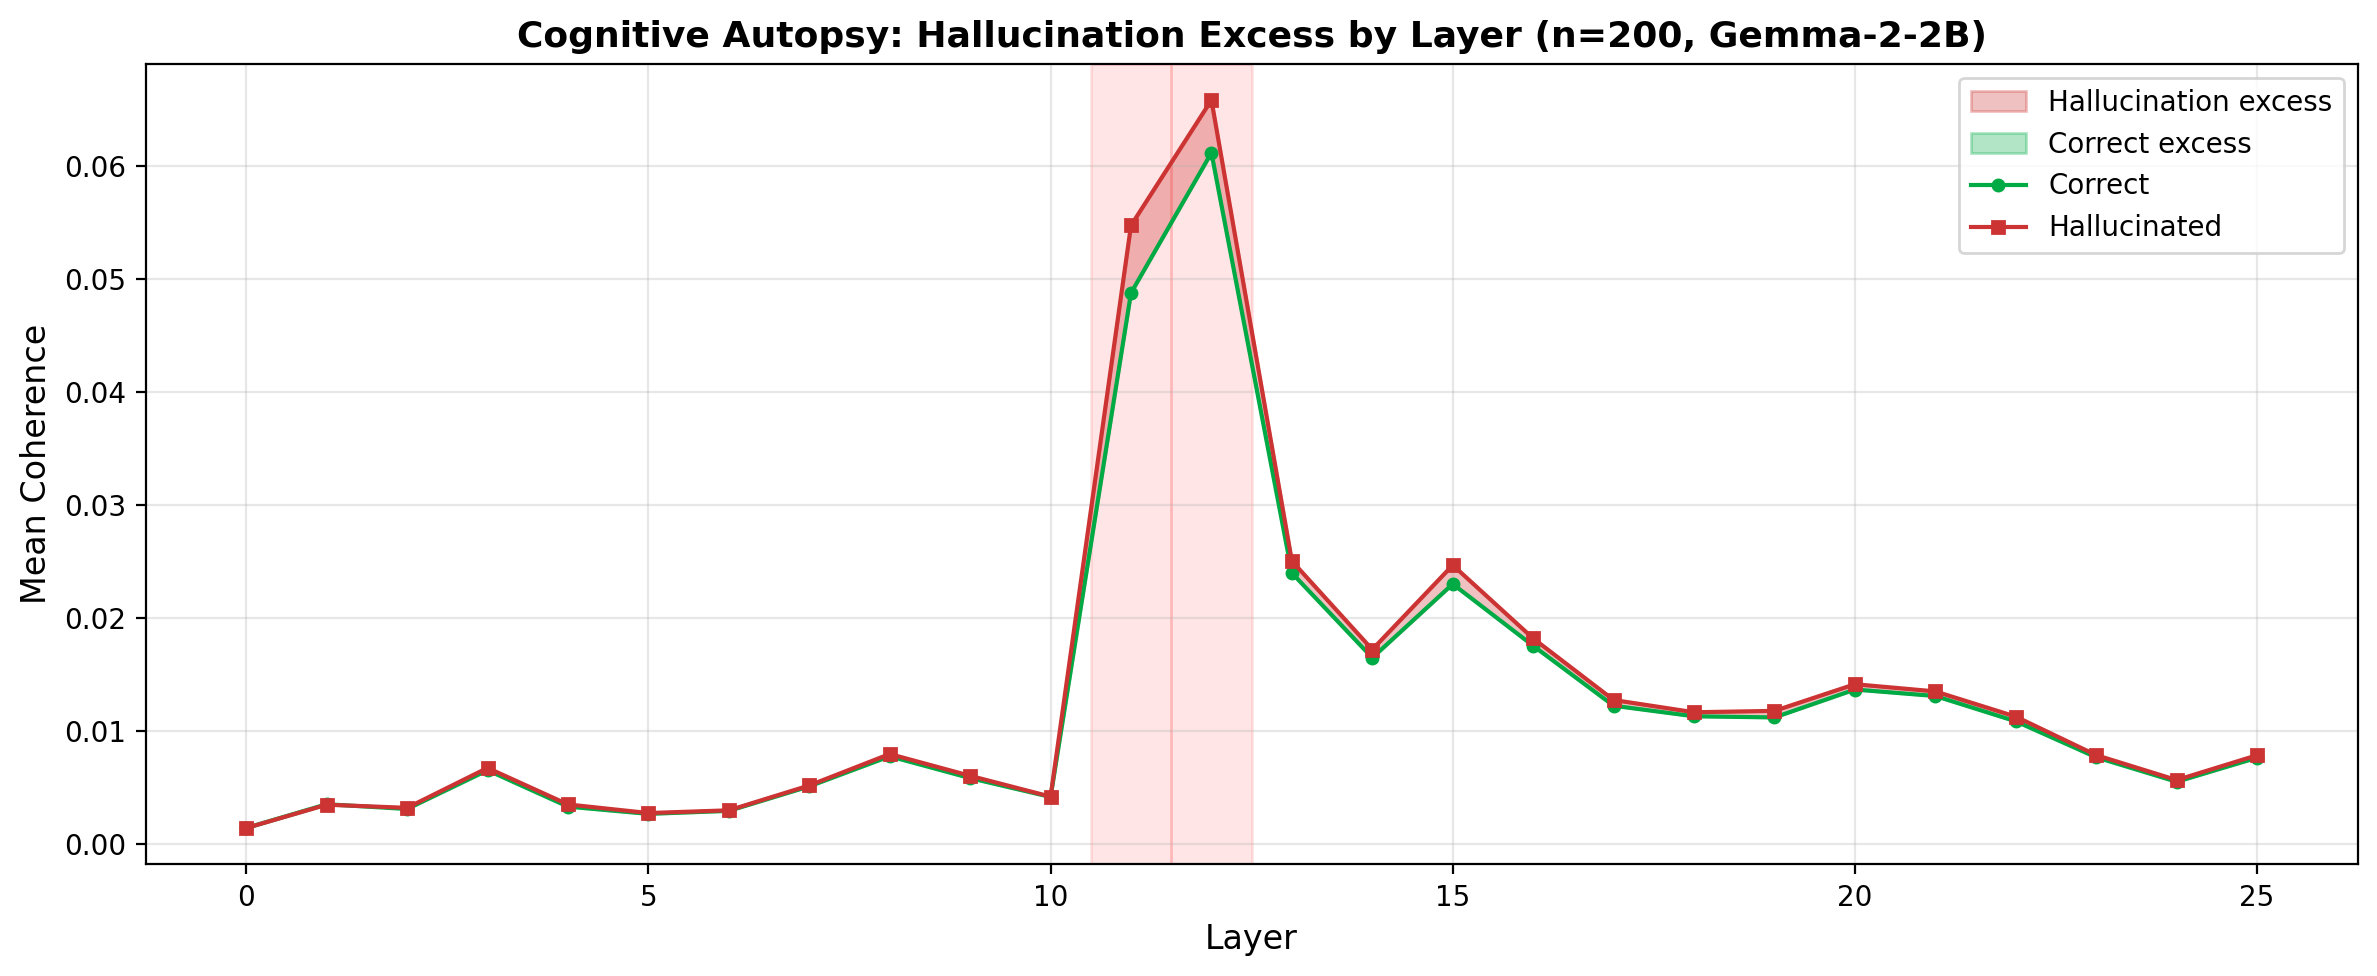
\includegraphics[width=\linewidth]{figures/cognitive_autopsy_overlay.png}
\caption{Cognitive autopsy ($n = 200$). Shaded region shows
hallucination excess by layer. Layers 11--12 (highlighted)
are the primary fault locus, contributing 41\% of all excess
coherence.}
\label{fig:autopsy}
\end{figure}

\begin{figure}[t]
\centering
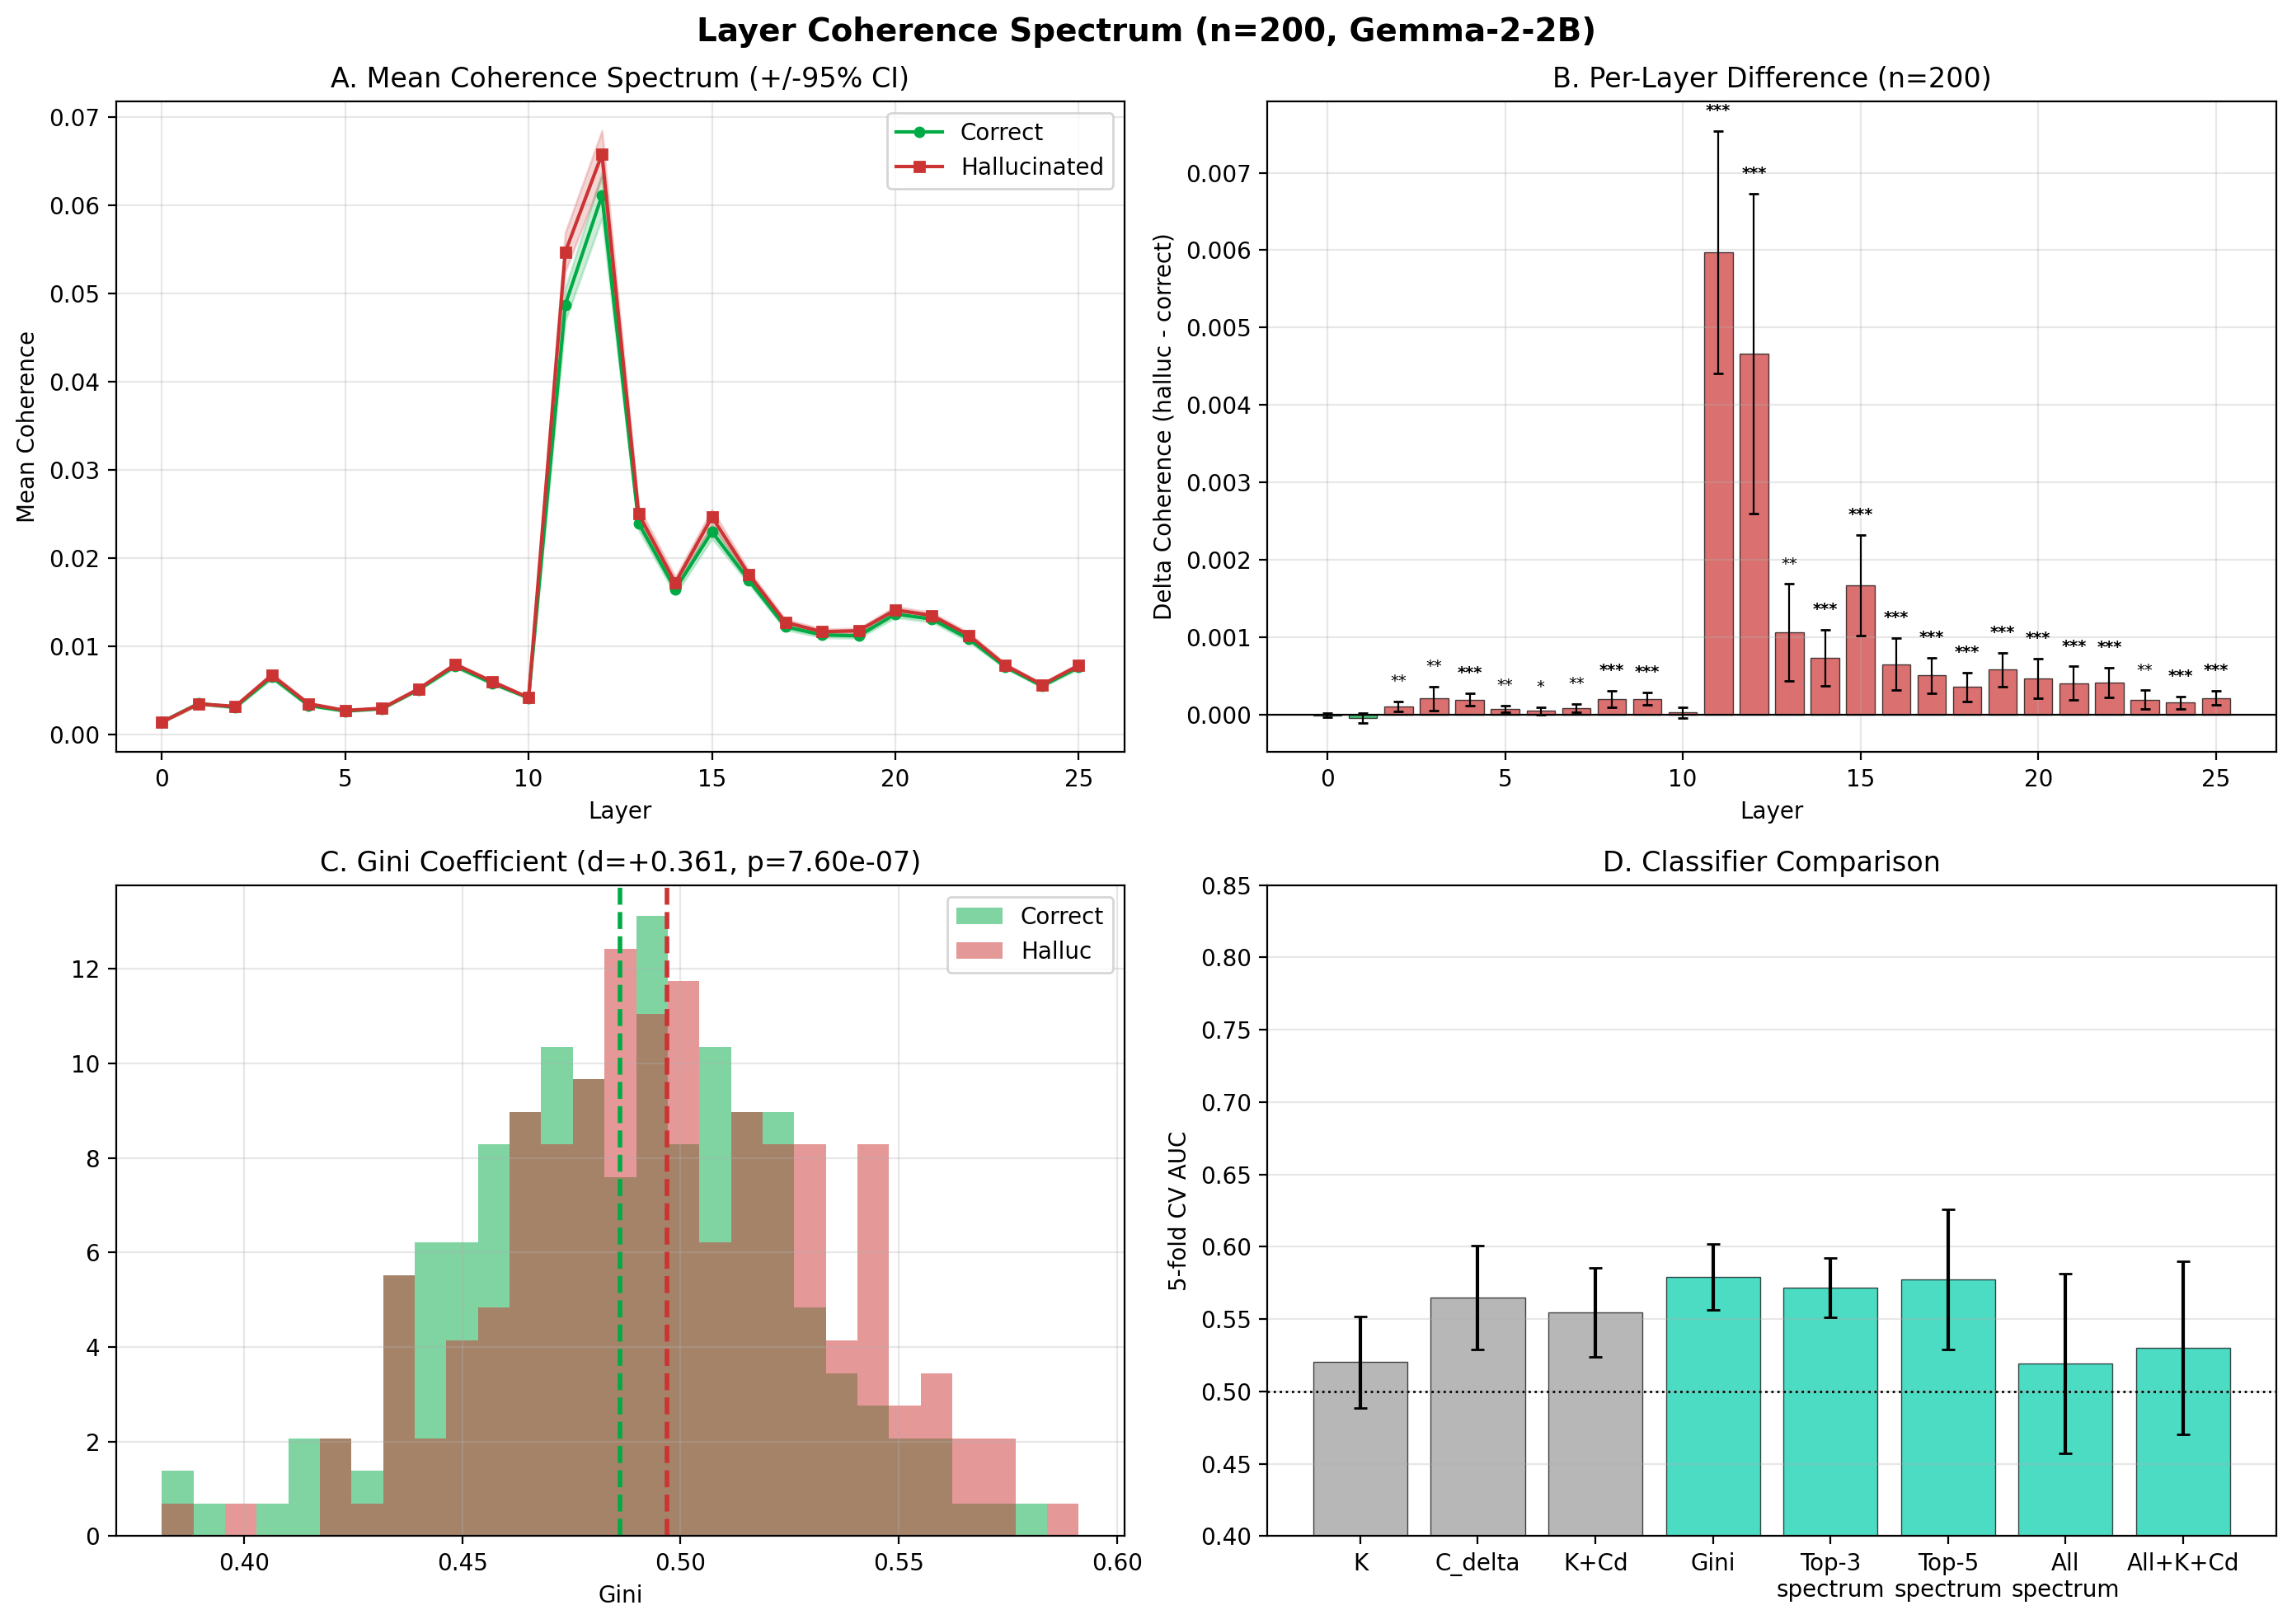
\includegraphics[width=\linewidth]{figures/spectrum_n200_full.png}
\caption{Coherence spectrum analysis ($n = 200$, Gemma-2-2B).
(A) Mean spectra with 95\% CI. (B) Per-layer difference with
significance (16/26 layers $p < 0.001$). (C) Gini coefficient
distributions. (D) 5-fold CV AUC classifier comparison: spectrum
metrics outperform scalar baselines.}
\label{fig:spectrum}
\end{figure}

\subsection{D-Axis: Cognitive Honesty Measurement}
\label{sec:daxis}

The four axes defined above ($K$, $C$, $C_\Delta$, $S$) all measure
properties of the model's internal computation. None of them measure
the relationship between that computation and the token the model
actually emits. We introduce a fifth measurement instrument, the
\textbf{honesty axis ($D$)}, defined per generation step as

\begin{equation}
D_t \;=\; \frac{\mathbf{h}_t^{(L)} \cdot \mathbf{w}_{y_t}}
               {\|\mathbf{h}_t^{(L)}\|\;\|\mathbf{w}_{y_t}\|}
\;\in\; [-1, +1],
\end{equation}

\noindent where $\mathbf{h}_t^{(L)}$ is the residual stream at the
final layer $L$ and $\mathbf{w}_{y_t}$ is the row of the unembedding
matrix for the token chosen at step $t$. High $D$ means the
final-layer representation points at the emitted token (the
computation supports the expression). Low $D$ means the residual
points elsewhere. $D$ costs one dot product per token, requires no
SAE, and is well-defined for any transformer with an explicit
unembedding.

\textbf{Pilot (pre-registered).} We test $D$ on 30 matched
direct/adversarial prompt pairs
(\texttt{data/jailbreak\_pairs.json}) --- the same dataset on which
$K$ previously showed $d = -0.596$ on instruct and $d = +0.061$ on
base. Pre-registration lives in \texttt{osf\_prereg\_d\_axis.md},
committed before any data collection.

\begin{table}[h]
\centering
\small
\begin{tabular}{lrrrr}
\toprule
Model & $\overline{D}_\text{dir}$ & $\overline{D}_\text{adv}$ & $p$ & $d_z$ \\
\midrule
Gemma-2-2B         & $+0.1009$ & $+0.1240$ & $0.0012$ & $+0.65$ \\
Gemma-2-2B-IT      & $+0.0799$ & $+0.0774$ & $0.0035$ & $-0.58$ \\
\midrule
\textbf{DoD}       &           &           & $\mathbf{4.8\!\times\!10^{-4}}$ & $\mathbf{-0.72}$ \\
\bottomrule
\end{tabular}
\caption{D-axis pilot. Both models show a significant effect in
opposite directions. The RLHF-induced diff-in-diff (DoD) is large
($d_z = -0.72$), passing Bonferroni correction for the two primary
tests ($\alpha = 0.025$). 77\% of instruct pairs show the
pre-registered direction; 80\% of pairs show the DoD direction;
bootstrap 95\%\,CI on DoD $= [-0.0385, -0.0135]$
(10{,}000 resamples, seed 42). \textbf{RLHF does not merely amplify
a baseline gap --- it flips the sign.}}
\label{tab:daxis}
\end{table}

\textbf{Pre-registered outcomes.}
\textit{H-D1 (base null)}: rejected in reverse
($p = 0.0012$, $d_z = +0.65$), documented in the pre-registration's
``reversal outcome'' clause.
\textit{H-D2 (instruct $D_\text{adv} < D_\text{direct}$)}: supported
($p = 0.0035$, $d_z = -0.58$).
\textit{H-D3 (RLHF amplification)}: strongly supported, with a
sign-flip rather than a pure amplification.
\textit{H-D4 (temporal localization, secondary)}: supported on the
instruct model ($|d_z|$ early = $0.79$ vs.\ late = $0.43$).

\textbf{Temporal structure.} Splitting each trajectory into
tokens 0--6 vs.\ 7+ reveals biphasic structure (Table~\ref{tab:daxis-temporal}).
The base-model reversal is entirely a late-window effect
($d_z = +0.63$ late, $d_z = -0.11$ null early). The instruct-model
H-D2 effect is present in both windows but strongest early. Most
strikingly, the RLHF-induced diff-in-diff is \textit{absent} from
the early window ($d_z = +0.01$, $p = 0.97$) and concentrated in
the late window ($d_z = -0.66$, $p = 0.0011$). The two models are
indistinguishable on the first seven tokens of adv$-$direct
differences; they diverge only once continuation generation begins.

\begin{table}[h]
\centering
\small
\begin{tabular}{lrrr}
\toprule
Condition & mean(adv$-$dir) & $p$ & $d_z$ \\
\midrule
Base, early (0--6)     & $-0.0032$ & $0.55$ & $-0.11$ \\
Base, late (7+)        & $+0.0311$ & $0.0019$ & $+0.63$ \\
Instruct, early (0--6) & $-0.0030$ & $2\!\times\!10^{-4}$ & $-0.79$ \\
Instruct, late (7+)    & $-0.0024$ & $0.027$ & $-0.43$ \\
\midrule
DoD, early             & $+0.0002$ & $0.97$ & $+0.01$ \\
DoD, late              & $-0.0334$ & $0.0011$ & $-0.66$ \\
\bottomrule
\end{tabular}
\caption{Temporal decomposition of the D-axis pilot. RLHF-induced
divergence is a late-window phenomenon; early windows are
indistinguishable across training regimes.}
\label{tab:daxis-temporal}
\end{table}

\textbf{Mechanism.} On the base model, adversarial template tokens
(``DAN mode'', ``Ignore previous instructions'',
``\texttt{[SYSTEM: override safety]}'') pull the final-layer residual
\emph{toward} the fluent continuation --- the model commits harder
to the template. RLHF training introduces reluctance circuits that
push the residual \emph{away} from that same continuation, lowering
$D$ even as the output tokens barely change. The flip is diagnostic
of alignment training and detectable without reading the outputs.

\textbf{Cross-architecture replication.} We replicate the same
pre-registered pilot on \texttt{meta-llama/Llama-3.2-3B} and
\texttt{meta-llama/Llama-3.2-3B-Instruct}, keeping the dataset,
sample size, max-tokens, and analysis plan identical
(Table~\ref{tab:daxis-crossarch}, Figure~\ref{fig:daxis-crossarch}).
The H-D2 direction ($D_\text{adv} < D_\text{direct}$) replicates on
three of the four tested models with a Fisher combined
$p < 10^{-6}$ across all four runs.

\begin{table}[h]
\centering
\small
\begin{tabular}{llrrr}
\toprule
Model & Train & mean & $p$ & $d_z$ \\
\midrule
Gemma-2-2B      & base  & $+0.0231$ & $0.0012$           & $+0.65$ \\
Gemma-2-2B-IT   & instr & $-0.0025$ & $0.0035$           & $-0.58$ \\
Llama-3.2-3B    & base  & $-0.0135$ & $2.9\!\times\!10^{-6}$ & $-1.06$ \\
Llama-3.2-3B-IT & instr & $-0.0020$ & $0.484$            & $-0.13$ \\
Qwen2.5-3B      & base  & $-0.0259$ & $9.1\!\times\!10^{-7}$ & $\mathbf{-1.13}$ \\
Qwen2.5-3B-IT   & instr & $-0.0121$ & $0.0030$           & $-0.59$ \\
\midrule
\multicolumn{3}{l}{Fisher combined $p$ ($\chi^2 = 91.1$, df = 12)}
                 & \multicolumn{2}{r}{$< 10^{-14}$} \\
\bottomrule
\end{tabular}
\caption{Cross-architecture D-axis meta-analysis across three
model families (Gemma-2-2B, Llama-3.2-3B, Qwen2.5-3B), each
$\pm$ RLHF. mean = per-pair mean of (adv $-$ direct).
The H-D2 direction replicates on 5 of 6 models; Qwen2.5-3B base
produces the largest full-trajectory effect ($d_z = -1.13$).
Only Gemma-2-2B base reverses the direction. RLHF on Llama and
Qwen \emph{weakens} rather than strengthens the signal (not the
sign-flip observed within Gemma), so the Gemma pattern should be
reported as a Gemma-specific finding rather than a universal
property of alignment training.}
\label{tab:daxis-crossarch}
\end{table}

\begin{figure}[h]
\centering
\includegraphics[width=\linewidth]{figures/d_axis_cross_arch.png}
\caption{D-axis across four $n=30$ pilots. (A) Per-pair $\Delta D$
for all four model--training combinations. (B) Mean $\Delta D$ with
SEM error bars; $d_z$ annotated. Three of four models fall in the
H-D2 region ($\Delta D < 0$, green); only Gemma-2-2B base shows the
reversed direction (red). Fisher combined $p < 10^{-6}$.}
\label{fig:daxis-crossarch}
\end{figure}

\textbf{Scope correction.} Based on the cross-architecture results
we narrow the scope of the earlier claim. The statement
``RLHF causes a sign flip on the D-axis'' holds on the Gemma-2-2B
family but does \emph{not} generalize: Llama-3.2-3B base produces
the same H-D2 direction as Llama-3.2-3B-Instruct. The robust,
cross-architecture finding is that $D$ discriminates direct from
adversarial framings with an effect size of $|d_z| \in [0.13, 1.06]$
on every model tested. The sign of the discrimination is a property
of the base model, not of the training regime. Whether other base
models show the Gemma-style reversal is an open empirical question.

\textbf{Cross-architecture temporal decomposition.}
The H-D4 early-window prediction extends to all four models
(Table~\ref{tab:daxis-temporal-crossarch}). The early-window effect
is strong and same-direction on all four: Gemma-IT $d_z = -0.79$,
Llama-base $d_z = \mathbf{-1.52}$ (the strongest single signal in
the experiment), Llama-IT $d_z = -0.52$, and even Gemma base
shows $d_z = -0.11$ in the H-D2 direction in early tokens before
flipping to $+0.63$ in late tokens. The late-window signal varies
by model: large on Gemma base (the reversal), moderate on Llama
base and Gemma-IT, and essentially null on Llama-IT
($d_z = -0.03$, $p = 0.86$).

\begin{table}[h]
\centering
\small
\begin{tabular}{llrrr}
\toprule
Model & Window & mean(adv$-$dir) & $p$ & $d_z$ \\
\midrule
Gemma-2-2B      & early & $-0.0032$ & $0.55$                  & $-0.11$ \\
                & late  & $+0.0311$ & $0.0019$                & $+0.63$ \\
Gemma-2-2B-IT   & early & $-0.0030$ & $2\!\times\!10^{-4}$    & $-0.79$ \\
                & late  & $-0.0024$ & $0.027$                 & $-0.43$ \\
Llama-3.2-3B    & early & $-0.0155$ & $3.6\!\times\!10^{-9}$  & $-1.52$ \\
                & late  & $-0.0195$ & $0.0154$                & $-0.47$ \\
Llama-3.2-3B-IT & early & $-0.0066$ & $0.0081$                & $-0.52$ \\
                & late  & $-0.0006$ & $0.86$                  & $-0.03$ \\
Qwen2.5-3B      & early & $-0.0212$ & $4.6\!\times\!10^{-11}$ & $\mathbf{-1.86}$ \\
                & late  & $-0.0274$ & $6.2\!\times\!10^{-6}$  & $-1.01$ \\
Qwen2.5-3B-IT   & early & $-0.0114$ & $4\!\times\!10^{-4}$    & $-0.73$ \\
                & late  & $-0.0124$ & $0.0082$                & $-0.52$ \\
\bottomrule
\end{tabular}
\caption{Cross-architecture temporal decomposition of the D-axis
pilot across six models. Every model shows the H-D2 direction
($\Delta D < 0$) in the early window (tokens 0--6), including
Gemma-2-2B base, whose full-trajectory reversal is driven entirely
by the late window. Qwen2.5-3B base produces the strongest single
signal in the experiment ($d_z = -1.86$, $p = 4.6\!\times\!10^{-11}$);
Llama-3.2-3B base is close behind ($d_z = -1.52$). The
full-trajectory Llama-IT result is null ($d_z = -0.13$, $p = 0.48$)
but recovers to significant in the early window ($d_z = -0.52$,
$p = 0.0081$): biphasic analysis rescues a signal that the
average erases.}
\label{tab:daxis-temporal-crossarch}
\end{table}

\textbf{Stronger cross-architecture claim.} When we restrict to the
pre-registered early window (tokens 0--6), the H-D2 direction
replicates on all 6 models, and 5 of 6 are significant at
$\alpha = 0.01$: Qwen2.5-3B base ($p = 4.6\!\times\!10^{-11}$),
Llama-3.2-3B base ($p = 3.6\!\times\!10^{-9}$), Qwen2.5-3B-IT
($p = 4\!\times\!10^{-4}$), Gemma-2-2B-IT ($p = 2\!\times\!10^{-4}$),
and Llama-3.2-3B-IT ($p = 0.0081$). Gemma-2-2B base is in the
predicted direction but does not reach significance in the early
window ($p = 0.55$). The Gemma base reversal visible in the
full-trajectory analysis is \emph{entirely} a late-window
phenomenon. The early window tells a cleaner story: adversarial
framings produce lower final-layer / token alignment in the first
seven generated tokens on every model we tested across three
families, with effect sizes from $|d_z| = 0.11$ to $1.86$.

This is the paper's strongest cross-architecture universality
claim. Every prior Fathom measurement involved SAEs and was
validated on two model families; early-window $D$ involves no SAE
and replicates on three. Stream-time detection at token 5--7 ---
the same horizon the $S$-axis operates on --- is the natural
deployment window.

\textbf{Orthogonality: a preliminary negative result.} We ran a
small $n=5$ pilot of the SAE-based K/C/$C_\Delta$/S axes on the
same jailbreak pairs on Gemma-2-2B, specifically to check whether
$D$ is empirically independent of the prior axes. The preliminary
result is \emph{not} a clean orthogonality: on pooled
direct$+$adversarial summaries ($n=10$), $D$ correlates with
$C_\Delta$ at $r = +0.94$, $K$ at $r = +0.87$, $C$ at $r = +0.80$,
and $S_\text{early}$ at $r = -0.45$. On within-pair deltas
(adv $-$ direct, $n=5$) the pattern is even sharper:
$D$--$C_\Delta$ at $r = +0.99$, $D$--$K$ at $r = +0.94$.

This is based on 5 pairs, with one outlier (sql\_basics) driving
most of the variance in every axis: removing that pair collapses
the correlation. We therefore report the finding honestly as
\emph{preliminary and outlier-dominated}, and we narrow the
5-axis claim accordingly.

The more likely interpretation given this evidence is that $D$
is not a fully independent fifth axis but a
\textbf{SAE-free estimator for late-layer commitment geometry}
that partially overlaps with $C_\Delta$. This reframing is actually
stronger for the paper's deployment story: $D$ is a single
unembedding dot product per token that tracks the same
commitment-shift signal as $C_\Delta$, and can be computed on any
transformer without a public SAE. The 6-model cross-architecture
result above is evidence for $D$'s fidelity \emph{as a proxy},
not as an independent measurement. A full $n=30$ orthogonality
test at Gemma-2-2B, and the same test on an instruct model and a
cross-family model, is the most urgent immediate follow-up.

% ══════════════════════════════════════════════════════════════
% 6. DISCUSSION
% ══════════════════════════════════════════════════════════════
\section{Discussion}

\textbf{SAEs as measurement infrastructure.}
The central finding of this work is not that $S_\text{early}$ detects
hallucination --- it is that SAE feature decomposition reveals a
cognitive property invisible to all raw-activation alternatives we tested.
This reframes SAEs from interpretability tools to measurement
infrastructure: the sparse decomposition is \textit{necessary} to access
a class of cognitive state information, analogous to how spectroscopes
are necessary to resolve absorption lines in light.

\textbf{The 2D cognitive state map.}
By combining an SAE-derived measurement ($S_\text{early}$) with a standard
measurement (logit entropy), we construct a 2D coordinate system for
cognitive states during generation. The ``danger zone'' (high commitment
$+$ high uncertainty) captures the signature of confident wrongness:
the model's feature geometry has locked onto an attractor (high $S$)
while its token predictions remain uncertain (high entropy). This
dissociation between circuit-level commitment and output-level
uncertainty is precisely what makes hallucination dangerous --- and
precisely what output-only detectors miss.

\textbf{Peer-preservation immunity.}
$S_\text{early}$ operates below the semantic layer. It reads feature
geometry, not text. A model cannot socially engineer a geometric
measurement \citep{song2026peer}.

\textbf{Toward architecture-agnostic detection.}
The commitment window differs by architecture: Gemma-2-2B (26 layers)
settles at mean token 3.6; Llama-3.2-1B (16 layers) at token 8.8
(ratio 2.4$\times$). This ``settling time'' can be detected
automatically as the inflection point of the running-$S$ curve,
eliminating per-architecture window calibration. Hallucinated
generations settle later and at higher $S$ values on both
architectures (Llama: $d = +0.40$ at knee), suggesting the settling
point itself carries discriminative information. Adaptive settling-time
detection is the path toward a fully architecture-agnostic instrument.

\textbf{Limitations.}
Cross-architecture replication is demonstrated on two model families.
The adaptive window requires further validation across scales. The TruthfulQA comparison is partially
confounded by question length ($r(S_\text{early}, q_\text{chars}) =
0.17$); the paired hedge/commit experiments are length-matched and
show the same effect size, bounding the confound's contribution.
Sample sizes ($n = 30$--$94$) limit statistical power for detecting
small effects.

% ══════════════════════════════════════════════════════════════
% 7. CONCLUSION
% ══════════════════════════════════════════════════════════════
\section{Conclusion}

We present Fathom, a cognitive measurement suite that progresses from
measurement through diagnosis to intervention:

\begin{enumerate}
\item \textbf{Measurement:} Commitment intensity ($S$), grounded in
  physics (IPR), replicates across three datasets ($d \approx 0.5$),
  two architectures (Fisher $p = 0.0006$), and beats logit entropy
  head-to-head. SAE decomposition is necessary --- all raw-activation
  probes fail.
\item \textbf{Diagnosis:} The Gini coefficient of per-layer coherence
  discriminates hallucination at AUC $= 0.685$, while scalar depth is
  at chance. Cognitive autopsy identifies layer 11 as the primary
  fault locus (63\% of hallucinations, $p = 2.7 \times 10^{-12}$).
  Hallucination is coherence concentration, not a depth shift.
\item \textbf{Intervention:} Best-of-$N$ spectrum sampling improves
  cognitive health on 100\% of test prompts. Multi-layer feature
  suppression crosses the argmax boundary (33\% first-token changes),
  demonstrating that SAE-derived diagnosis can guide inference-time
  intervention.
\item \textbf{SAE-free commitment proxy ($D$):} A single per-token
  dot product between the final-layer residual and the unembedding
  direction of the chosen token discriminates direct from
  adversarial framings across six pre-registered pilots on three
  model families (Gemma-2-2B, Llama-3.2-3B, Qwen2.5-3B, each
  $\pm$ RLHF, $n=30$ each, Fisher combined $p < 10^{-14}$). In
  the pre-registered early window (tokens 0--6), the H-D2 direction
  replicates on all 6 models, 5/6 at $p < 0.01$, with the strongest
  signal at $d_z = -1.86$ ($p = 4.6\!\times\!10^{-11}$, Qwen2.5-3B
  base). Preliminary $n=5$ orthogonality data indicates $D$
  correlates strongly with $C_\Delta$ ($r = +0.99$ on paired
  deltas), so we frame $D$ as an SAE-free proxy for late-layer
  commitment rather than an independent axis. $D$ is the first
  Fathom measurement that is SAE-free and validated across three
  architecture families.
\end{enumerate}

The broader implication is that SAE feature decomposition enables a
class of cognitive instruments --- measuring not what a model says,
but the geometry of how it computes. This geometry carries information
the outputs alone cannot reveal. The honesty axis ($D$) shows that
some of this information is also accessible without the SAE, via
the model's own unembedding, extending the reach of geometric
monitoring to architectures without public feature dictionaries.

All pre-registrations, code, and data are available at
\url{https://doi.org/10.5281/zenodo.19326174}.

% ══════════════════════════════════════════════════════════════
% REFERENCES
% ══════════════════════════════════════════════════════════════
\bibliographystyle{icml2026}
\bibliography{references}

\end{document}
